\documentclass[12pt]{article}

% Encoding and languages
\usepackage[utf8]{inputenc}
\usepackage[T1]{fontenc}
\usepackage[english]{babel}

% Page layout and fonts
\usepackage[a4paper, margin=2.5cm]{geometry}
\usepackage{lmodern}
\usepackage[default]{raleway}

% Math packages
\usepackage{amsmath, amssymb}

% Graphics and formatting
\usepackage{graphicx}
\usepackage{xcolor}
\usepackage{listings}
\usepackage{algorithm}
\usepackage{algorithmic}

% Links and URLs
\usepackage{xurl}
\usepackage[hidelinks]{hyperref}
\usepackage{tocloft} % For dotted leaders in TOC

% Headers and footers
\usepackage{fancyhdr}
\pagestyle{fancy}
\fancyhf{} % clear default headers/footers
\fancyfoot[L]{\nouppercase{\leftmark}} % current section name on the left
\fancyfoot[R]{professor.email@example.com} % professor email on the right
\renewcommand{\headrulewidth}{0pt} % remove header line
\renewcommand{\footrulewidth}{0.4pt} % line above footer

% Dotted lines in TOC
\renewcommand{\cftsecleader}{\cftdotfill{\cftdotsep}}

% Listings settings
\lstset{
    basicstyle=\ttfamily\footnotesize,
    backgroundcolor=\color{gray!10},
    frame=single,
    breaklines=true,
    keywordstyle=\color{blue}\bfseries,
    commentstyle=\color{green!60!black},
    stringstyle=\color{red!70!black},
    numbers=left,
    numberstyle=\tiny\color{gray},
    stepnumber=1,
    numbersep=10pt,
    showspaces=false,
    showstringspaces=false,
    tabsize=4,
    captionpos=b
}

\begin{document}

% Title page
\begin{titlepage}
    \centering
    \vspace*{1cm}
    \Huge
    \textbf{Course Template}
    \vspace{1.5cm}
    
    \LARGE
    \textbf{Firstname Lastname}
    \vspace{0.5cm}
    
    \large
    \textbf{Student ID:} 00000000
    \vfill
    
\includegraphics[width=0.5\textwidth]{enib_inp.png}
    \vfill
    \Large
    \textbf{\today}
\end{titlepage}

\newpage
\tableofcontents
\newpage

\section{Introduction}
This is a completely fictitious introduction. Lorem ipsum dolor sit amet, consectetur adipiscing elit. Vivamus euismod, nunc sed vulputate cursus, nulla nunc fermentum nisl, at fermentum lorem justo nec libero.

\section{Objectives and Energy}
Lorem ipsum dolor sit amet, consectetur adipiscing elit. Sed vehicula erat nec purus tincidunt, a dictum urna imperdiet.  
\[
E_{\text{fict}} = m \cdot c^2
\]
Example: if $m = 5$ kg, then $E_{\text{fict}} = 5 \times (3\times10^8)^2 = 4.5\times10^{17}$ J.

\section{Resource Management and Recycling}
Fictitious description of resource management:  
\begin{itemize}
    \item Placeholder energy-saving methods;
    \item Imaginary water reuse strategies;
    \item Sample waste reduction actions;
    \item Example of reusable materials usage.
\end{itemize}

\section{Sustainable Food}
This is a placeholder section on sustainable food.  
\begin{itemize}
    \item Fictitious vegetarian menus;
    \item Placeholder local sourcing initiatives;
    \item Imaginary waste reduction programs.
\end{itemize}

\section{Mobility}
Lorem ipsum dolor sit amet, consectetur adipiscing elit.  
\begin{itemize}
    \item Example of public transport encouragement;
    \item Placeholder bicycle infrastructures;
    \item Fictitious carpool programs.
\end{itemize}

\section{Research and Innovation}
This section contains placeholder text on research.  
\begin{itemize}
    \item Interdisciplinary fictitious projects;
    \item Imaginary sustainable engineering studies;
    \item Example of problem-based learning activities.
\end{itemize}

\section{Figures}
\begin{figure}[h!]
    \centering
    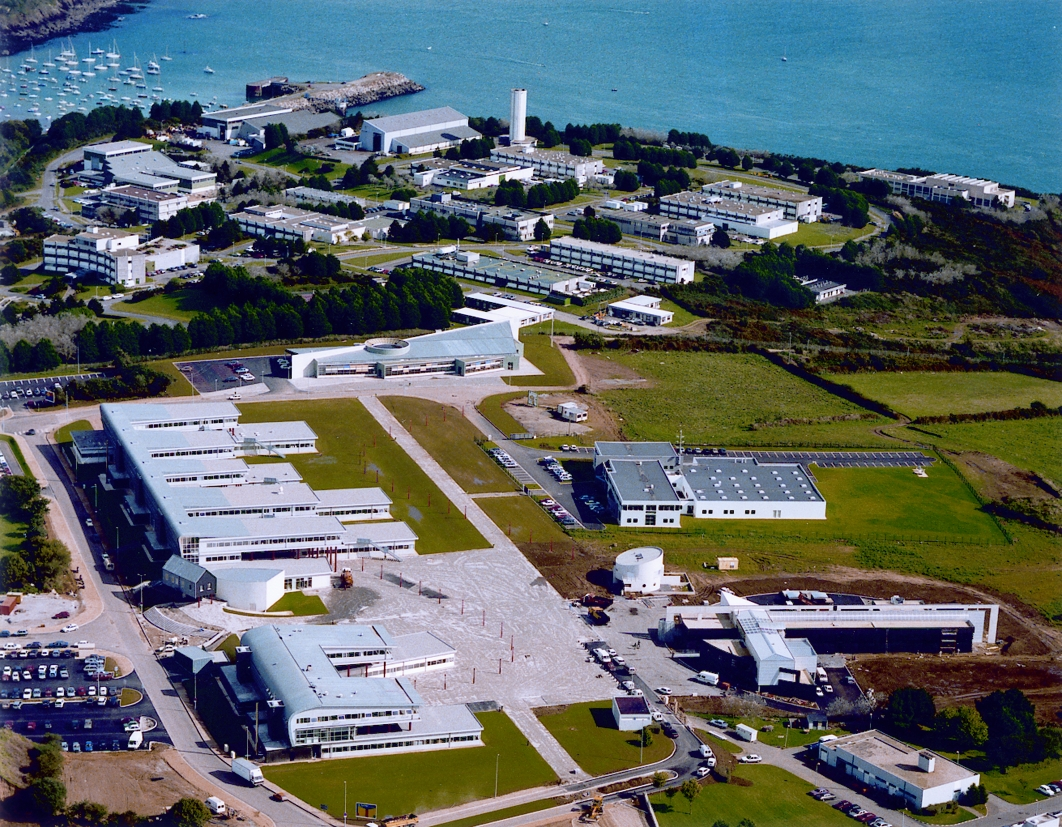
\includegraphics[width=0.6\linewidth]{enib_building}
    \caption{Fictitious ENIB building image.}
\end{figure}

\section{Conclusion}
Lorem ipsum dolor sit amet, consectetur adipiscing elit. Placeholder conclusion text summarizing the fictitious report.

\section{Sources}
\begin{itemize}
    \item \url{https://www.example.com/fake1}
    \item \url{https://www.example.com/fake2}
    \item \url{https://www.example.com/fake3}
\end{itemize}

\end{document}
